\chapter{Suffix arrays}\label{ch:suffix-arrays}
Een tweede datastructuur die we in meer detail bekijken zijn suffix arrays.
Dit doen we omwille van de lagere geheugenvereisten in vergelijking met suffixbomen.

\section{Wat zijn suffix arrays?}\label{sec:wat-zijn-suffix-arrays?}
Suffix arrays zijn een geheugenefficiëntere voorstelling van suffixbomen.
In plaats van een boomstructuur maken we hier gebruik van \textbf{een array die de volgnummers van elke suffix in de originele string bevat}.
Deze volgnummers worden lexicografisch gesorteerd op basis van de overeenkomstige suffix.
Figuur~\ref{fig:suffixtree_vs_suffixarray} geeft een voorbeeld van een suffixboom en suffix array opgebouwd over de tekst \texttt{acacgt\$}.

\begin{center}
    \texttt{tekst: a|c|a|c|g|t|\$\\index: 0|1|2|3|4|5|6}
\end{center}
\begin{figure}[H]

    \begin{subfigure}[b]{0.6\linewidth}
        \resizebox{\linewidth}{!}{
            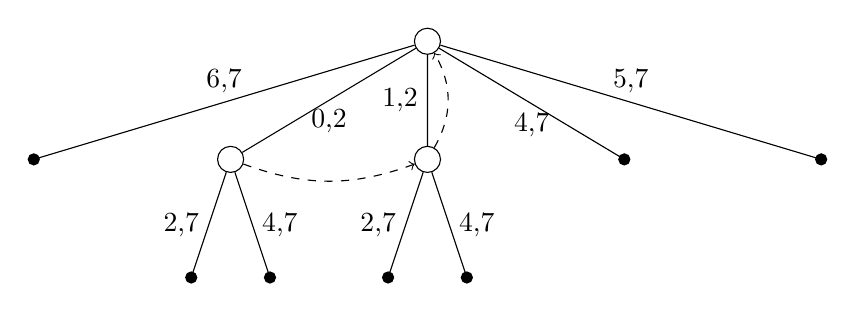
\begin{tikzpicture}
            [
                level 1/.style = {sibling distance = 2.5cm},
                level 2/.style = {sibling distance = 1cm}
            ]

                \node[draw, circle] (End2) {}
                child {
                    [fill] circle (2pt)
                    edge from parent node [above] {6,7}
                }
                child {
                    node[draw, circle] (Start1) {}
                    child {
                        [fill] circle (2pt)
                        edge from parent node [left] {2,7}
                    }
                    child {
                        [fill] circle (2pt)
                        edge from parent node [right] {4,7}
                    }
                    edge from parent node [below] {0,2}
                }
                child {
                    node[draw, circle] (End1) {}
                    child {
                        [fill] circle (2pt)
                        edge from parent node [left] {2,7}
                    }
                    child {
                        [fill] circle (2pt)
                        edge from parent node [right] {4,7}
                    }
                    edge from parent node [left] {1,2}
                }
                child {
                    [fill] circle (2pt)
                    edge from parent node [below] {4,7}
                }
                child {
                    [fill] circle (2pt)
                    edge from parent node [above] {5,7}
                }
                ;
                \draw[dashed, ->] (Start1) to[out=-20,in=200] (End1);
                \draw[dashed, ->] (End1) to[out=60,in=-60] (End2);
            \end{tikzpicture}
        }
        \caption{Suffixboom}
    \end{subfigure}
    \begin{subfigure}[b]{0.4\linewidth}
        \centering
        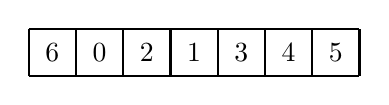
\begin{tikzpicture}[thick,scale=.6]
            \draw (0,0) grid (7,1);
            \path (.5,.5) node{$6$} foreach \i in {0,2,1,3,4,5} {++(1,0) node{$\i$}};
        \end{tikzpicture}
        \vspace{3em} % vertically center the array a bit
        \caption{Suffix array}
    \end{subfigure}

    \caption{Suffixboom en suffix array voor de string \texttt{acacgt\$}.}\label{fig:suffixtree_vs_suffixarray}
\end{figure}

Wanneer we de bladeren van de suffixboom van links naar rechts bekijken zien we dat dit overeen komt met de suffix array.
Dit is de link tussen deze twee datastructuren.
Merk op dat \textbf{de suffix array minder data bevat ten opzichte van de suffixboom}.
De interne knopen en suffix links uit de suffixboom ontbreken.
Indien deze informatie ook nodig is kan gebruik maakt worden van zogenaamde Enhanced Suffix Arrays (ESAs).
Hierbij worden naast de suffix array nog drie extra tabellen bijgehouden.
Deze worden de Longest Common Prefix (LCP), Child en suffix link table genoemd.

\section{Complexiteit}\label{sec:complexiteit}
Traditionele sorteeralgoritmes zoals merge sort~\cite{mergeSort} kunnen in $O(n \log n)$ tijd en $O(n^2)$ geheugen een suffix array opbouwen.
Hierbij is $n$ de lengte van de tekst.
Ondertussen bestaan er echter verschillende algoritmes die een tijdscomplexiteit van $O(n)$ bereiken~\cite{sais, ko_alura, radixSA, dark_archon, libdivsufsort}.
Bovendien vereisen deze veel minder geheugen dan een equivalente suffixboom.
Sommige implementaties vereisen slechts $5n + O(1)$ geheugen~\cite{dark_archon, libdivsufsort}.


\section{Bestaande implementaties}\label{sec:bestaande-implementaties}
Aangezien er meerdere sterk geoptimaliseerde implementaties bestaan voor het opbouwen van een suffix array vergelijken we eerst de performantie van deze implementaties.
Hieruit kunnen we nadien een snelle en geheugenefficiënte implementatie selecteren.
Tabel~\ref{tab:sa_building} bevat een overzicht van verschillende algoritmes.
Voor sommige werden verschillende implementaties getest.

\begin{table}[H]
    \begin{minipage}{\linewidth}
        \centering
            \begin{tabular}{l l S[table-format=-2.2] S[table-format=-2.2] S[table-format=-1.2] S[table-format=-1.2]}
                Algoritme & Programmeertaal & \multicolumn{2}{c}{Tijd (in s)} & \multicolumn{2}{c}{Geheugen (in GB)} \\
                \hline\hline
                &                      & {32 bit} & {64 bit} & {32 bit} & {64 bit} \\
                \cline{3-6}
                libdivsufsort\footnote{\url{https://github.com/y-256/libdivsufsort}}                                       & C                    & 15.01    & 15.97    & 1.03     & 1.86     \\
                libdivsufsort\footnote{\url{https://github.com/baku4/libdivsufsort-rs}}                                    & Rust + bindings to C & 16.00    & 15.52    & 1.03     & 1.86     \\
                libdivsufsort\footnote{\url{https://github.com/fasterthanlime/stringsearch/tree/master/crates/divsufsort}}  & Rust                 & 20.23    & {-}      & 1.03     & {-}      \\
                dark archon a4\footnote{\url{https://github.com/kvark/dark-archon}}                                        & C                    & 39.34    & {-}      & 1.09     & {-}      \\
                libsais\footnote{\url{https://github.com/IlyaGrebnov/libsais}}                                             & C                    & 6.38     & 6.46     & 1.03     & 1.86     \\
                SA-IS\footnote{\url{https://github.com/Tascate/Suffix-Arrays-in-CPP}}                                      & C++                  & 24.39    & {-}      & 3.80     & {-}      \\
                SA-IS\footnote{\url{https://github.com/sile/sais}}                                                         & C++                  & 18.73    & {-}      & 1.46     & {-}      \\
                radixSA\footnote{\url{https://github.com/mariusmni/radixSA64}}                                             & C++                  & 9.74     & 11.26    & 2.11     & 3.52     \\
                \hline
            \end{tabular}
        \caption{Uitvoeringstijd en maximaal geheugenverbruik voor het opbouwen van een suffix array aan de hand van verschillende algoritmes voor de Swiss-Prot eiwitdatabank.
        Indien er een 32 bit en 64 bit integer implementatie beschikbaar was werden deze allebei getest. Een - staat voor niet getest. Deze testen werden lokaal uitgevoerd op een M1 Pro MacBook Pro. De specificaties hiervan zijn terug te vinden in tabel~\ref{tab:macbook_hardware}.}
        \label{tab:sa_building}
    \end{minipage}
\end{table}

We kunnen concluderen dat \textbf{libsais duidelijk de snelste implementatie is om Swiss-Prot te indexeren}.
\textbf{Samen met libdivsufsort gebruikt het de kleinste hoeveelheid geheugen}, wat libdivsufsort ook interessant maakt.
Een ander voordeel dat libsais en libdivsufsort hebben, naast hun minimale geheugenverbruik, is dat ze allebei een 64 bit integer implementatie hebben.
Dit is belangrijk voor het indexeren van UniprotKB omdat de totale tekst langer is dan het grootste 32 bit integer.
Dit zorgt ervoor dat alle 32 bit integer implementaties onbruikbaar zijn voor dit einddoel.
Tot slot valt ook te zien dat het verschil tussen de C en Rust versie die bindings heeft naar de C code klein is.
De overhead van het oproepen van de C code uit Rust is dus minimaal.

\subsection{Enhanced suffix arrays}\label{subsec:enhanced-suffix-arrays}
Om een indicatie te hebben van de extra hoeveelheid geheugen die nodig is om gebruik te maken van Enchanced Suffix Arrays kunnen we via de libsais bibliotheek de pCLP en LCP array berekenen.
Deze LCP array is slechts één van de drie extra tabellen die deel zijn van ESAs, maar het is voor ons wel de meest interessante.
De baseline waarmee we willen vergelijken is de hoeveelheid geheugen dat we nodig hebben om enkel se SA op te bouwen.
Voor de Swiss-Prot eiwitdatabank was dit 2.3 GB\@.
Als we ook de pLCP array berekenen is het maximale geheugengebruik 4.43 GB RAM, en met de LCP array loopt dit zelfs op naar 5.72 GB\@.
\textbf{Het berekenen van deze extra arrays vraagt dus ongeveer dubbel zo veel geheugen, waardoor we deze optie niet verder uitwerken}.
Bovendien lost de LCP array ons probleem nog niet op.
Op basis van de SA en LCP array moeten nog een compacte representatie van de boomstructuur gevonden worden.
Dit is niet vanzelfsprekend.

\section{Toepassen van suffix arrays op een eiwitdatabank}\label{sec:toepassen-van-suffix-arrays-op-een-eiwitdatabank}
Het moeilijkste deel van onze probleemstelling is het opbouwen van de suffix array.
Dit kunnen we oplossen aan de hand van de algoritmes uit sectie~\ref{sec:bestaande-implementaties}.
Eens we die suffix array opgebouwd hebben blijft er echter nog een stuk van ons probleem over.
Eerst moeten we nog een mapping maken van de gevonden suffixen naar het bijbehorende eiwit.
Op basis van dit eiwit wordt daarna de LCA gezocht.

\subsection{Bouwen van de suffix array}\label{subsec:bouwen-van-de-suffix-array}
Zoals in de inleiding van sectie~\ref{sec:probleemstelling} willen we Rust gebruiken vanwege de combinatie van \textit{memory safety} en hoge performantie.
We willen echter gebruik maken van de al bestaande geoptimaliseerde algoritmes om een suffix array op te bouwen.
Om beide doelen te bereiken maken we gebruik van interoperabiliteit tussen Rust en C/C++.
Zo bestaan er al bindings\footnote{\url{https://crates.io/crates/libdivsufsort-rs}} van Rust naar de originele implementatie van libdivsufsort\cite{libdivsufsort} (in C).
Ook al blijkt uit het testen dat dit algoritme voor het opbouwen van de indexstructuur over een kleinere eiwitdatabank niet het snelste is.
Het geheugengebruik is wel minimaal.
Dit laat toe om te experimenteren met het opbouwen van een SA zonder al te veel extra werk, en al onmiddellijk te zien hoe het geheugengebruik evolueert.
\\ \\
Later hebben zelf nog een simple Rust wrapper geschreven rond de libsais C code.
Dit gebruik makende van het \texttt{bindgen}\footnote{\url{https://crates.io/crates/bindgen}} crate.
Op deze manier is het ook mogelijk om gebruik te maken van de snellere libsais algoritme eens we wisten dat SAs een efficiënte en schaalbare oplossing waren voor de probleemstelling.
\\ \\
Het nadeel van het gebruiken van deze bindings naar C code is dat het oproepen van de effectieve C code gebeurt in een \texttt{unsafe} blok.
Hierbij is het dus mogelijk dat er geheugenfouten in het programma sluipen.
Dit risico is echter miniem aangezien dit bestaande, geteste bibliotheken zijn.
Bovendien zijn we ook zeker dat eventuele geheugenfouten enkel hierdoor kunnen ontstaan.
Dit is dus een afweging tussen optimale performantie (waarbij we het wiel niet hoeven heruit te vinden), en garantie van \textit{memory safety}.

\subsection{Mapping van suffix naar proteïne}\label{subsec:mapping-van-suffix-naar-proteine}
Bepalen welke proteïne hoort bij een bepaalde suffix kan op twee manieren.
\textbf{Een eerste optie, laten we deze een \textit{dense mapping} noemen, is om expliciet voor elke suffix bij te houden bij welke proteïne die hoort}.
Dit kan aan de hand van een array die even lang is als het aantal suffixen.
Het voordeel van deze aanpak is dat het vinden van de bijbehorende proteïne in $O(1)$ tijd kan, hiervoor is echter wel $O(m)$ geheugen nodig, met $m$ de lengte van de totale tekst.
\\ \\
\textbf{De tweede optie, aan de hand van een \textit{sparse mapping}, is om enkel de eerste of laatste suffix per proteïne bij te houden}.
Het voordeel van deze aanpak is dat er minder geheugen nodig is, meer precies $O(n)$ geheugen met $n$ het aantal proteïnen.
Het nadeel is dan weer dat het vinden van de bijbehorende proteïne trager is.
Dit neemt $O(\log n)$ tijd in beslag aan de hand van binair zoeken.
Hierbij is $n$ het aantal proteïnes.
\\ \\
In Figuur~\ref{fig:dense_vs_sparse} wordt de uitvoeringstijd voor beide implementaties vergeleken.
\textbf{Standaard (en in alle komende testen) zullen wij gebruik maken van de \textit{sparse mapping} aangezien de performantie impact in de praktijk beperkt is, en er een significante hoeveelheid geheugengebruik uitgespaard kan worden}.
Zo loopt het verschil in geheugengebruik op tot 0.8 GB voor Swiss-Prot.
Dit is maar liefst 25\% van de indexgrootte bij de \textit{dense mapping}.
Het grote verschil in uitvoeringstijd bij het Human-Prot peptidebestand valt te verklaren vanwege het extreem hoog aantal matches dat daar te vinden is voor de korte peptides.
In de praktijk zullen we dit maximaal aantal matches echter limiteren (zie sectie~\ref{subsec:maximaal-aantal-matches}).
Dit zal op zijn beurt ook de overhead van de sparse mapping beperkt houden.
\begin{figure}[H]
    \centering
    \subfloat[Tijd nodig om alle matches te zoeken.]{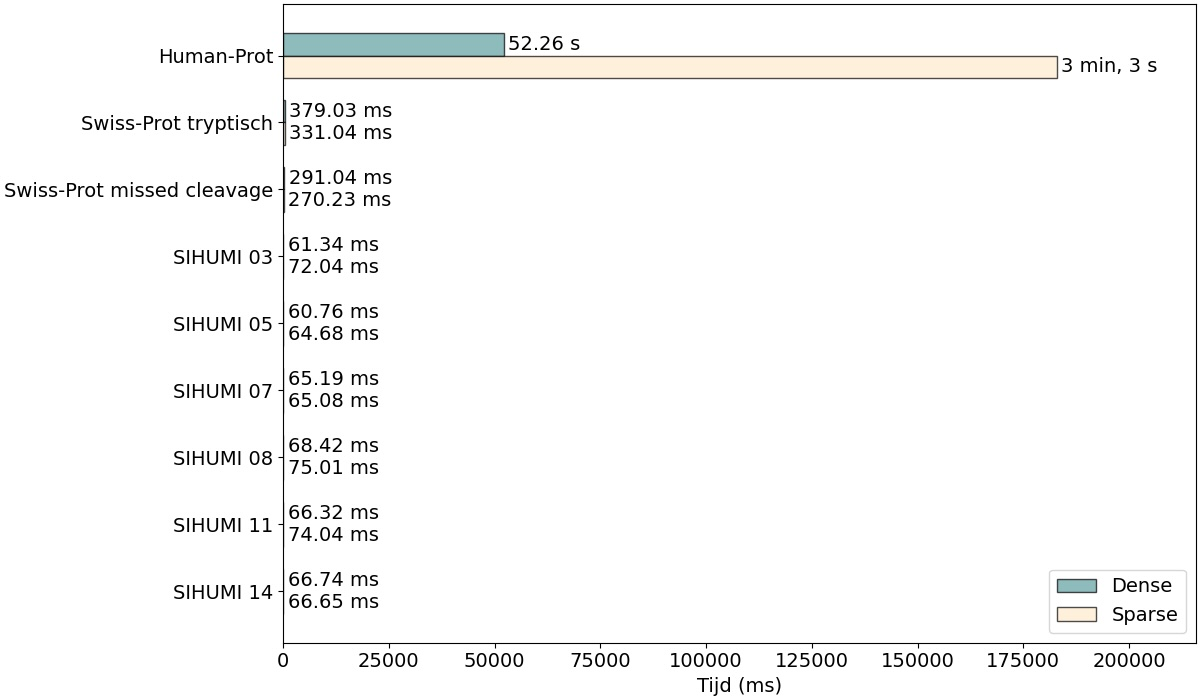
\includegraphics[width=\linewidth]{dense_vs_sparse_time}}\\[4ex] % [4ex] om wat extra vertical spacing in te voegen

    \subfloat[Maximaal gebruikt geheugen tijdens het zoeken naar alle matches.]{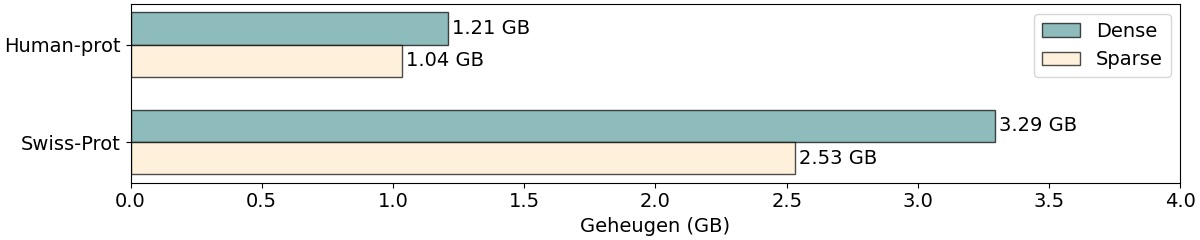
\includegraphics[width=\linewidth]{dense_vs_sparse_memory}}
    \caption{Zoektijd en geheugengebruik bij het gebruik bij een \textit{dense} of \textit{sparse mapping} van de suffixen naar de proteïnes.}\label{fig:dense_vs_sparse}
\end{figure}

\subsection{Berekenen van de LCA}\label{subsec:berekenen-van-de-lca}
Zoals eerder vermeld, bevat een suffix array geen informatie over de interne toppen die voorkomen bij een suffixboom.
Dit zorgt ervoor dat het niet mogelijk is om op basis hiervan de LCA van de organismen voor te berekenen voor al deze interne toppen.
Dit moet nu \textit{on the fly} gebeuren tijdens het zoekproces zelf.
Hierdoor is er ook \textbf{geen reden meer om LCA te gebruiken in de plaats van LCA*}.
LCA* was namelijk onze eerste keuze omdat de geaggregeerde data bij deze heuristiek langer gedetailleerd blijft.
Bij suffixbomen zijn we daar echter van moeten afstappen om het voorberekenen efficiënter te maken.

\section{Sparse en compressed suffix arrays}\label{sec:sparse-en-compressed-suffix-arrays}
Om het geheugenverbruik van suffix arrays verder te verkleinen kan er gebruik gemaakt worden van sparse of compressed suffix arrays.
In principe doen ze allebei hetzelfde, er wordt namelijk slechts een stuk van de originele suffix array bijgehouden.
Het verschil zit in welk stuk bijgehouden wordt.
\\ \\
Sparse suffix arrays (SSAs) bouwen een suffix array op basis van elke k-de suffix van de input tekst.
Indien we slechts 50\% van de suffixen bijhouden komt dit er op neer dat enkel suffixen die beginnen op een \textbf{even index in de inputtekst} bijgehouden worden.
Bij compressed suffix arrays (CSAs) wordt daarentegen slechts elke k-de waarde van de SA bijgehouden.
Indien we in dit geval 50\% van de suffixen bijhouden komt dit er hier op neer dat enkel suffixen die op een \textbf{even index staan in de opgebouwde suffix array} over blijven
\\ \\
Voor beide opties is de populairste manier om ze op te bouwen aan de hand van \textbf{\textit{sampling} op de volledige SA\@}.
Hierdoor blijft het maximale geheugenverbruik tijdens het opbouwen identiek aan het gebruik van de volledige SA\@.
Dit is net het punt waar wij ons geheugenverbruik verder willen verlagen.
Gelukkig heeft het gebruik hiervan nog altijd het voordeel dat de uiteindelijke machine die de index zal hosten lagere geheugenvereisten zal hebben.
\\ \\
Het samplen van een opgebouwde suffix array is de meest gebruikte methode tot op vandaag vanwege de bestaande sterk geoptimaliseerde implementaties van de klassieke SA constructie algoritmes.
Bij sparse suffix arrays is het beste algoritme qua tijdscomplexiteit tot nu toe een Monte Carlo algoritme dat $O(n)$ tijd en $O(b)$ geheugen nodig heeft en een Las Vegas algoritme dat $O(n \sqrt{\log b})$ tijd en $O(b)$ geheugen verbruikt.
Hierbij is $n$ de lengte van de tekst, en $b$ het aantal effectief gebruikte suffixes in de sparse SA~\cite{building_sparse_sa}.
Van het Monte-Carlo algoritme is er een bestaande implementatie\footnote{\url{https://github.com/lorrainea/SSA/tree/main/MA}}.
Wanneer we aan de hand hiervan een SSA met sparseness factor 3 voor Swiss-Prot opbouwen blijkt dit niet alleen trager te zijn ($\pm$ 10 minuten).
Ook het geheugengebruik ligt merkelijk hoger ($\pm$ 10 GB).
Terwijl we slechts een tiental seconden nodig hebben om de standaard SA op te bouwen in combinatie met 1.8 GB RAM\@.
Voor compressed suffix arrays bestaat er een algoritme dat een tijdscomplexiteit van $o(n)$ heeft in combinatie met $O(n \log \sigma)$ bits aan geheugen~\cite{building_compressed_sa}.
Hierbij is $n$ de tekstlengte en $\sigma$ de alfabetgrootte.
\\ \\
Het grootste nadeel aan deze algoritmes in context van deze thesis is dat er nog geen sterk geoptimaliseerde implementaties bestaan.
Bovendien zal de \textbf{factor van ingevoegde sparseness in ons geval altijd vrij klein} zijn om de zoektijden beperkt te houden (aangezien we werken met een erg grote dataset en vrij korte strings).
Indien we dus een implementatie hebben om rechtstreeks een CSA of SSA te bouwen, maar met een grotere constante qua geheugengebruik zal vanwege de kleine sparseness factor de winst snel verloren gaan.
\textbf{In ons geval is een SSA interessanter dan een CSA} omwille van de verschillende restricties tijdens het zoeken dat een SSA en CSA hebben.
\\ \\
Bij het gebruik van sampling factor $k$ kunnen we bij een SSA alle sequenties van lengte $k$ en groter zoeken.
Bij een CSA is het mogelijk dat ook sommige sequenties die groter zijn dan $k$ niet te vinden zijn, en sommige kortere wel.
Dit omdat het mogelijk is dat er in het slechtste geval een gat van $n - \frac{n}{k}$ suffixen zit tussen twee opeenvolgende bijgehouden suffixen in de CSA\@.
Hierbij is $n$ de lengte van de invoertekst.
Het zoeken van extreem korte sequenties is echter niet interessant omdat deze erg weinig informatie bevatten, terwijl het verliezen van enkele langere sequenties (zonder te kunnen voorspellen welke) net extra informatieverlies met zich meebrengt.
\\ \\
Bovenstaand probleem kan opgelost worden door gebruik te maken van extra datastructuren.
Zo kan een FM-index~\cite{fm_index} gebruik maken van een CSA, en kunnen we hierbij wel alle sequenties zoeken.
Om dit te doen moeten we echter tijdens het opbouwen van de indexstructuur nog bijkomende onderdelen berekenen (zoals de BWT\footnote{Burrows–Wheeler transformatie} van de tekst).
Dit verhoogt opnieuw het geheugengebruik tijdens het opbouwen.

\subsection{Zoeken in sparse suffix arrays}\label{subsec:zoeken-in-sparse-suffix-arrays}
Het zoeken in een SSA is erg gelijkaardig aan het zoeken in een volledige SA\@.
Een belangrijke \textbf{restrictie} is echter dat in de SSA \textbf{geen strings gezocht kunnen worden die kleiner zijn dan de sparseness factor}.
Bovendien heeft deze sparseness factor ook impact op de zoekperformantie.
Bij het zoeken met sparseness factor $k$ moeten we $k$ verschillende iteraties uitvoeren.
In iteratie $i$ gaan de eerste $i - 1$ tekens van de zoekstring overslaan.
In plaats van de zoekstring zoeken we dus een suffix van de zoekstring in de indexstructuur.
\\ \\
Voor elke matchende suffix (stel dat dit suffix $s$ is) moet daarna gecontroleerd worden als de overgeslagen prefix van $p$ tekens matcht met de $p$ tekens die op posities $[s - p, p[$ in de geïndexeerde tekst staan.
Als dit zo is, dan matcht suffix $s - p$ met de gezochte string.
Het eindresultaat is de unie van de resultaten van elke iteratie.
Om alles iets duidelijker te maken volgt een klein voorbeeld waarin we de peptide \texttt{acg} in de tekst \texttt{acacgt\$} zoeken.
De index die gebruikt wordt om te zoeken is een SSA met sparseness factor 3.
Deze valt terug te vinden in figuur~\ref{fig:sparse_sa}.

\begin{center}
    \texttt{tekst: a|c|a|c|g|t|\$\\index: 0|1|2|3|4|5|6}
\end{center}
\begin{figure}[H]
    \hfill
    \begin{subfigure}[t]{0.45\linewidth}
        \centering
        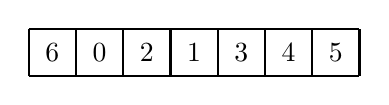
\begin{tikzpicture}[thick,scale=.6]
            \draw (0,0) grid (7,1);
            \path (.5,.5) node{$6$} foreach \i in {0,2,1,3,4,5} {++(1,0) node{$\i$}};
        \end{tikzpicture}
        \caption{Suffix array}
    \end{subfigure}
    \hfill
    \begin{subfigure}[t]{0.45\linewidth}
        \centering
        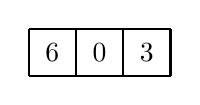
\begin{tikzpicture}[thick,scale=.6]
            \draw (0,0) grid (3,1);
            \path (.5,.5) node{$6$} foreach \i in {0,3} {++(1,0) node{$\i$}};
        \end{tikzpicture}
        \caption{Sparse suffix array met sparseness factor 3.}
    \end{subfigure}
    \hfill
    \caption{SA en SSA voor de tekst \texttt{acacgt\$}.}
    \label{fig:sparse_sa}
\end{figure}

\begin{enumerate}
    \item Sla 0 tekens over.
    Zoek \texttt{acg} in de SSA\@.
    We vinden geen matches.
    \item Sla 1 teken over.
    Dit wil zeggen dat we \texttt{cg} zoeken in de SSA\@.
    Dit levert een match op met suffix 3 (op index 1 in de SSA).
    \begin{enumerate}
        \item Controleer of de suffix die deels gematcht is ook volledig matcht met onze zoekstring.
        Dit wil zeggen dat we de overgeslagen prefix van $p = 1$ tekens (in dit geval de letter \texttt{a}) moeten kunnen matchen met de eerste $p$ tekens van suffix $3 - 1 = 2$.
        \item We zien dat het eerste teken van suffix 2 inderdaad een \texttt{a} is.
        Dit kan rechtstreeks via tekst gecontroleerd worden aan de hand van $p$ karakters die vergeleken moeten worden.
        Suffix 2 is dus een match voor de zoekstring \texttt{acg}.
    \end{enumerate}
    \item Sla 2 tekens over.
    Zoek \texttt{g} in de SSA\@.
    We vinden geen matches.
    \item We concluderen dat enkel suffix 2 matcht met de gezochte string \textit{acg}.
\end{enumerate}

\subsubsection{Performantie en indexgrootte}
Aangezien de sparseness factor impact heeft op de zoekperformantie is het belangrijk te zien hoe deze impact is, zodat we een goede keuze kunnen maken.
Op het eerste zicht lijkt het vergroten van deze factor enkel meer iteraties te vragen, maar dit heeft zware gevolgen.
Deze extra iteraties zullen ervoor zorgen dat er \textbf{kortere strings} in de SSA gezocht worden, die in het algemeen \textbf{meer matches} opleveren.
Voor al deze matches moeten we controleren of de tekens die ervoor komen matchen met de overgeslagen prefix.
Figuur~\ref{fig:search_sparseness}~(a) visualiseert de impact op de zoektijd van het Swiss-Prot peptidebestand met en zonder \textit{missed cleavages}.
Deze bestanden worden hiervoor gebruikt omdat de kortste sequentie die ze bevatten 5 aminozuren lang is.
Hierdoor blijft voor het gebruikte interval nog steeds elke peptide zoekbaar.
Bij het Human-Prot zoekbestand zijn er ook kortere peptides die we moeten overslaan, waardoor dit een slechte representatie is voor de evolutie van de zoektijd.
\\
\begin{figure}[H]
    \centering
    \subfloat[Zoektijd voor het Swiss-Prot peptidebestand met en zonder \textit{missed cleavages}. De zoekoperaties zijn uitgevoerd op een sparse suffix array gebouwd op basis van de Swiss-Prot eiwitdatabank.]{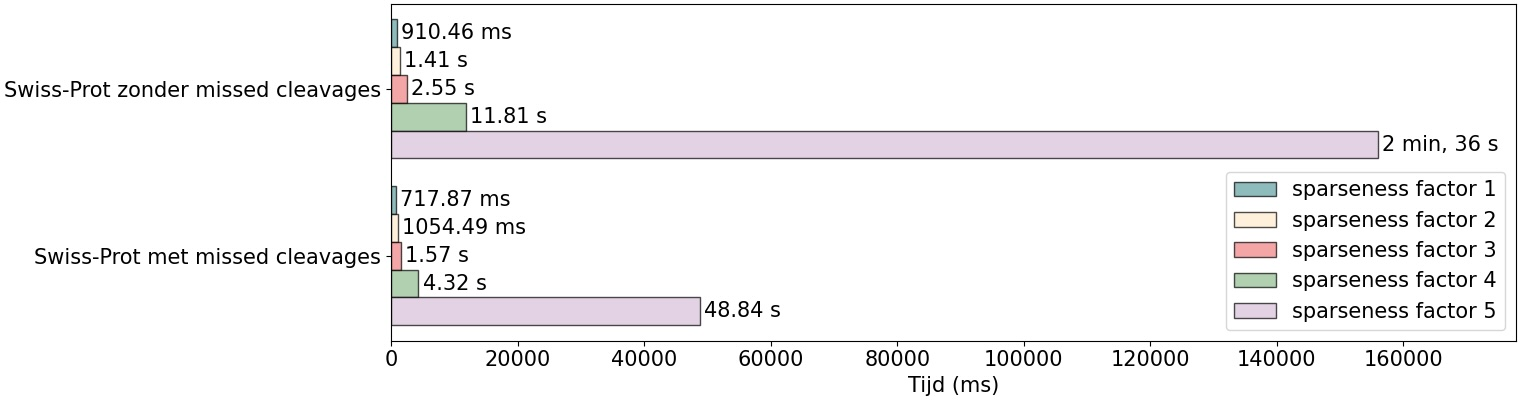
\includegraphics[width=\linewidth]{swissprot_searchtime_sparseness}}\\[4ex] % [4ex] om wat extra vertical spacing in te voegen

    \subfloat[Grootte van de volledige index en SSA voor de Swiss-Prot databank gebruik makende van verschillende sparseness factors.]{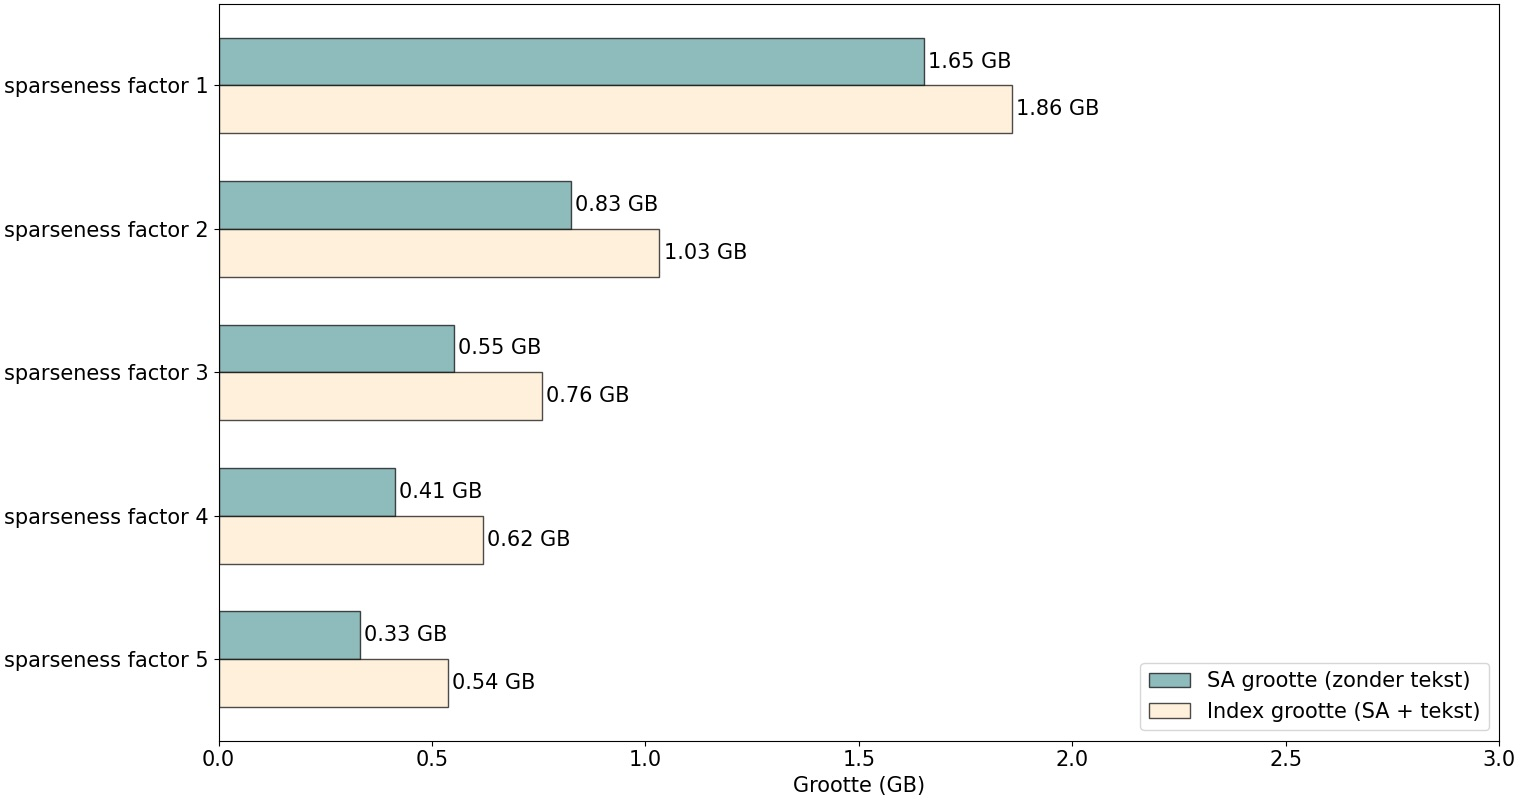
\includegraphics[width=0.8\linewidth]{index_size_SSA}}
    \caption{Zoektijd en indexgrootte voor Swiss-Prot.}\label{fig:search_sparseness}
\end{figure}

De zoektijd explodeert wanneer we de sparseness factor verhogen omdat een deel van de gezochte peptides bestaat uit 5 aminozuren.
Wanneer we deze proberen zoeken in een SSA met sparseness factor 5, zoeken we eigenlijk enkel één letter in de SSA (de laatste van de peptide).
Dit zal erg veel matches opleveren, en op zijn beurt erg veel werk vereisen om alle prefixen te controleren.
\\ \\
Anderzijds zal het verhogen van de sparseness factor de indexgrootte verkleinen.
Hierbij is het belangrijk dat enkel de SA mee verkleint.
Er blijft \textbf{altijd een vaste hoeveelheid geheugen nodig om de tekst zelf op te slaan}.
In Figuur~\ref{fig:search_sparseness}~(b) is duidelijk te zien dat, voor dit geval, de overgang van sparseness factor 4 naar 5 erg weinig winst heeft in opslag, maar een grote impact heeft op de performantie.
\\ \\
Er zijn dus twee erg belangrijke bevindingen over sparse suffix arrays, en de manier waarop wij ze opbouwen.
\begin{enumerate}
    \item Probeer de sparseness factor zo laag mogelijk te houden, zo blijft ook de zoektijd voor kortere peptiden beperkt.
    \item Het maximale geheugenverbruik blijft constant onafhankelijk van de sparseness factor.
    De hoeveelheid geheugen om ze nadien te gebruiken kunnen we wel verkleinen, hierdoor kan de index op lichtere machines gebruikt worden na het opbouwen.
\end{enumerate}

Dit impliceert dat we de factor enkel moeten verhogen om het geheugenverbruik te beperken bij een al opgebouwde indexstructuur.
Dit is vooral van toepassing voor UniProtKB waar het nuttig is om kort een krachtige machine te gebruiken die de SA bouwt, waarna een minder krachtige machine de SSA host.
In het perfecte geval wordt \textbf{de sparseness factor zo gekozen zodat de SSA samen met de tekst net in het RAM geheugen past} van deze minder krachtige machine.

\section{Parallellisatie}\label{sec:parallellisatie}
Om het zoeken nog verder te versnellen kan gebruik gemaakt worden van parallellisatie.
We hebben namelijk een \textbf{groot aantal peptides} waarvoor we elke keer dezelfde \textbf{statische indexstructuur} moeten doorzoeken.
Rust maakt dit proces vrij simpel omdat het \textit{ownership} systeem dataraces voorkomt (behalve wanneer gebruik gemaakt wordt van \textit{unsafe} code of het \textit{interior mutability} patroon)\cite{rust_data_races}.
Om een datatype te gebruiken in combinatie met multithreading moet deze de \texttt{Sync} en \texttt{Send} trait implementeren.
Deze traits worden door het typesysteem automatisch afgeleid.
Namelijk, wanneer alle componenten van een type aan de \texttt{Sync} en \texttt{Send} trait voldoen, dan voldoet je nieuwe type ook automatisch.
\\ \\
Uiteindelijk hebben we twee geparallelliseerde implementaties gemaakt.
In de eerste wordt alles volledig zelf beheerd.
Hierbij verdelen we zelf welke data naar welke thread gaat, worden de threads manueel opgestart en sluiten we ze ook zelf af.
In de tweede implementatie wordt gebruik gemaakt van de Rayon crate\cite{rayon}.
Deze laat toe om op een simpele manier een sequentiële lus over een variabele te parallelliseren.
In ons geval was het omzetten van een sequentiële implementatie (nadat alle types voldeden aan de \texttt{Sync} en \texttt{Send} trait) zo simpel als het vervangen van \texttt{.iter()} door \texttt{.par\_iter()}.
Ook in deze implementatie is het mogelijk om manueel een specifiek aantal threads te kiezen.
Standaard gebruikt Rayon het aantal beschikbare logische cores op de machine, maar het instellen van een ander aantal kan aan de hand van één lijntje code.

\begin{minted}{Rust}
// Sequentieel
let results = peptides
    .iter()
    .map(|peptide| search_peptide(peptide))
    .collect();

// Parallel
let results = peptides
    .par_iter()
    .map(|peptide| search_peptide(peptide))
    .collect();
\end{minted}

\subsection{Manueel threaden vs Rayon}\label{subsec:manueel-threaden-vs-rayon}
Aangezien we twee verschillende implementaties hebben, is het interessant om na te gaan hoe deze allebei presteren.
Figuur~\ref{fig:threading_default_vs_rayon} toont de evolutie van de zoektijden voor een verschillend aantal threads.
We zien duidelijk dat de versie die gebruikt maakt van \textbf{Rayon net iets sneller} is en dat beide implementaties ongeveer \textbf{lineair schalen}.
De schaling is niet perfect één op één ten opzichte van het aantal threads omdat het inlezen en uitschrijven van de output sequentieel blijft.
Het verschil in uitvoeringstijd valt mogelijks te verklaren aan de manier waarop de data verdeeld wordt over de threads.
In combinatie met een efficiëntere manier om de resultaten uit de threads te verwerken.
In de eigen implementatie kreeg elke thread simpelweg $\frac{1}{x}$ van alle peptides toegekend, met $x$ het aantal threads.
De resultaten moeten daarna aan de hand van enkele stappen uit de thread-scope gehaald worden zodat deze terug beschikbaar zijn voor de rest van het programma.
Rayon maakt gebruik van een ingewikkelder systeem aan de hand van \textit{work stealing}\cite{rayon_stealing} om de data over de threads te verdelen.
Verder is het ophalen van de resultaten ook veel simpeler.
Deze worden rechtstreeks ter beschikking gesteld alsof er geen parallellisme was.

\begin{figure}[H]
    \centering
    \subfloat[Absolute uitvoeringstijd voor een verschillend aantal cores.]{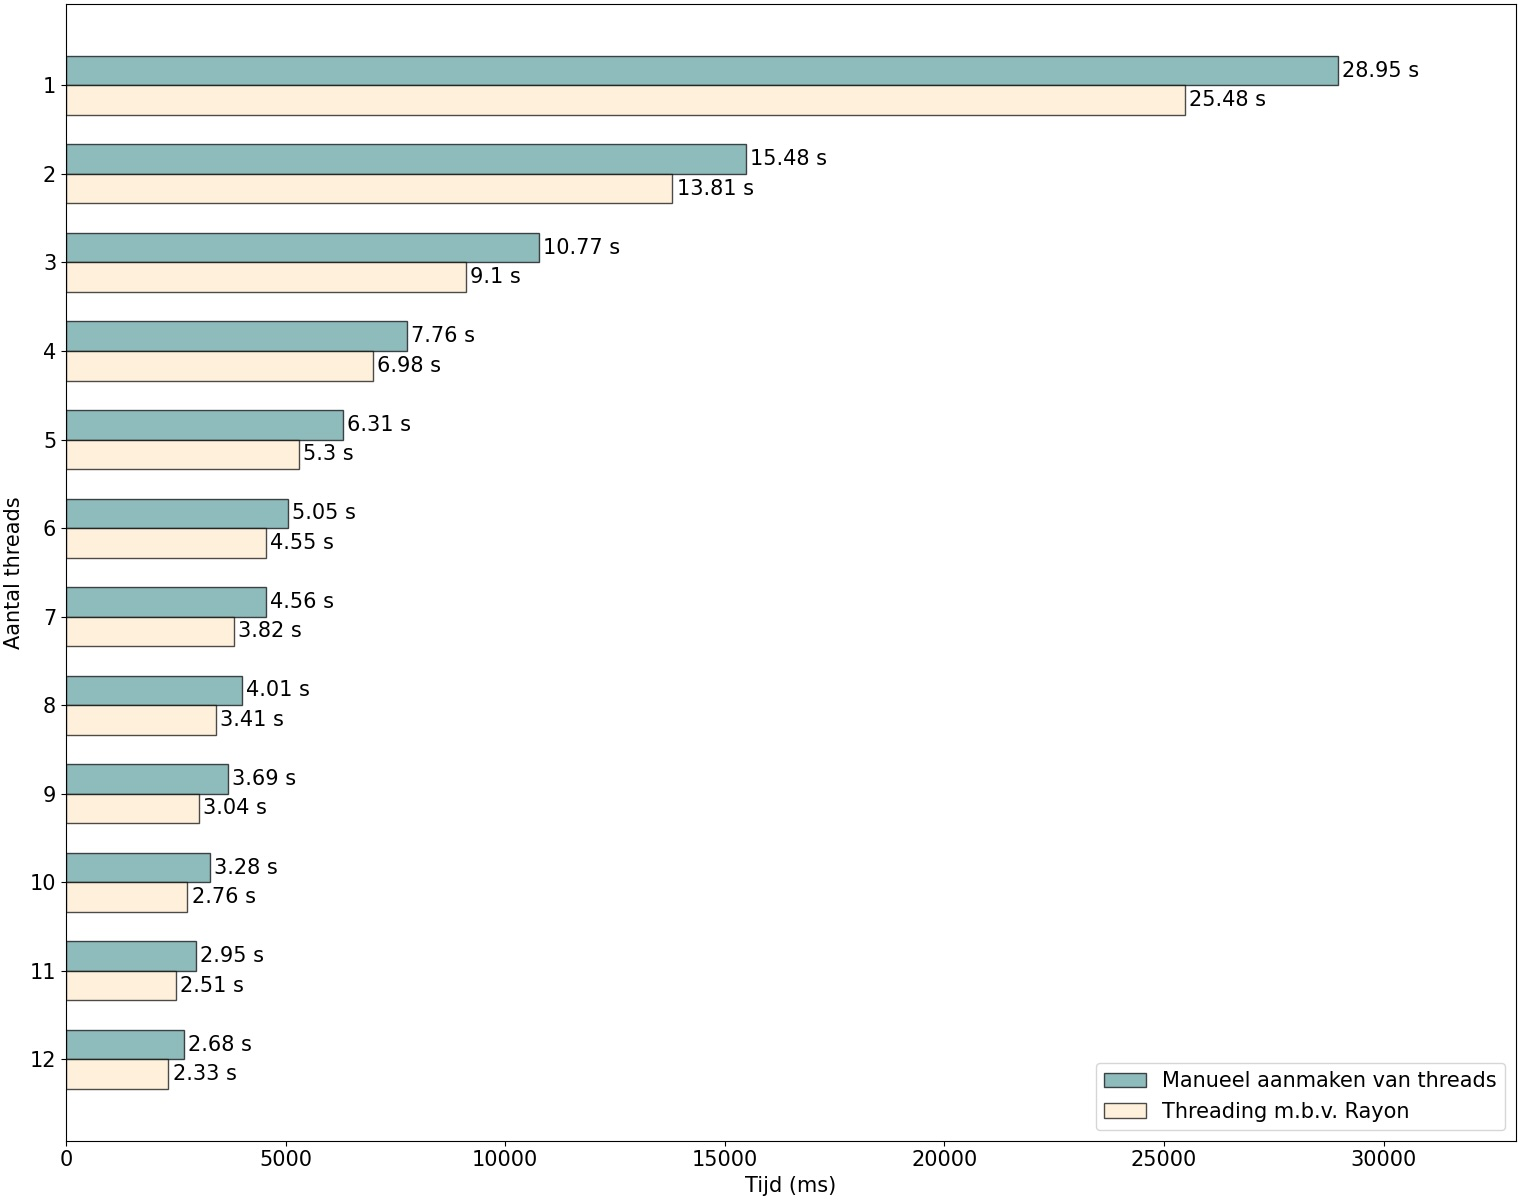
\includegraphics[width=0.7\linewidth]{threading_default_vs_rayon}}\\[4ex] % [4ex] om wat extra vertical spacing in te voegen

    \subfloat[Relatieve versnelling ten opzichte van uitvoering op 1 thread.]{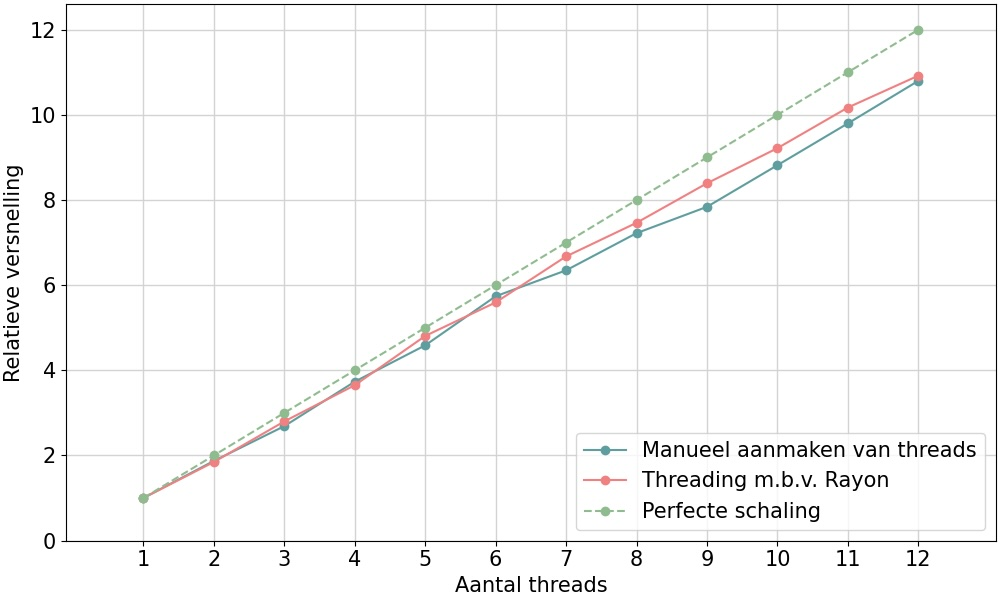
\includegraphics[width=0.7\linewidth]{threading_default_vs_rayon_relative}}
    \caption{Tijdsmeting om het Swiss-Prot peptidebestand zonder \textit{missed cleavages} te zoeken in een index met sparseness factor 3 ter grootte van 5\% van UniProtKB.}\label{fig:threading_default_vs_rayon}
\end{figure}

Naast het verschil in performantie zijn er nog andere voordelen verbonden aan het gebruik van Rayon.
De \textbf{code is namelijk veel simpeler en daarom ook beter te onderhouden}.
Dit motiveert onze keuze om finaal gebruik te maken van Rayon.

\section{Performantie}\label{sec:performantie}
Nu we verschillende manier verkend hebben om suffix arrays op te bouwen is het interessant om onze implementatie te vergelijken met suffixbomen.
Op basis hiervan kunnen we vaststellen welke verbeteringen we gemaakt hebben, of deze indexstructuur goed genoeg schaalt om toepasbaar te zijn op de volledige UniProtKB databank en in welke tijd de peptides gezocht kunnen worden.

\subsection{Opbouwen}
Figuur~\ref{fig:array_building} visualiseert de tijd nodig om de indexstructuur op te bouwen in combinatie met het geheugenverbruik.
Er is duidelijk een \textbf{mooie tijdswinst} verkregen, wat een bonus is voor het lokaal opbouwen van indices.
Voor het opbouwen van de index op UniProtKB is dit echter minder van belang aangezien dit proces slechts een vier tal keren per jaar moet gebeuren.
Zolang de nodige CPU tijd hiervoor niet langer is dan enkele dagen is dit acceptabel.
Een veel belangrijkere vaststelling is het \textbf{maximale geheugenverbruik tijdens opbouwen}.
Ook dit is \textbf{drastisch gedaald}.
Dit is exact de reden dat we deze indexstuctuur gekozen hebben.
Wanneer we het resultaat voor Swiss-Prot extrapoleren naar UniProtKB, gebruikmakende van de assumptie dat UniProtKB ongeveer 500 keer groter is dan is de verwachting dat er ongeveer 1.2 TB RAM nodig is.
Dit blijft een grote hoeveelheid aan geheugen, maar is wel al beschikbaar op de huidige generatie aan servers.
Zo bieden zowel Amazon via AWS, google via GCP en Microsoft via Azure instanties aan met enkele TB aan RAM\@.

\begin{figure}[H]
    \centering
    \subfloat[Tijd nodig om de index op te bouwen.]{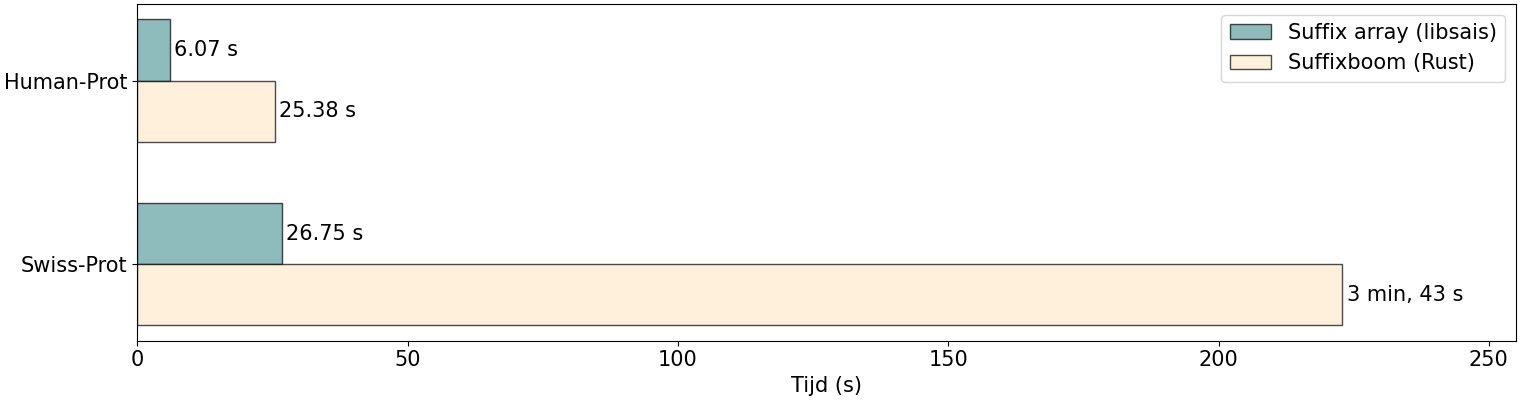
\includegraphics[width=\linewidth]{building_array_libsais_time}}\\[4ex] % [4ex] om wat extra vertical spacing in te voegen

    \subfloat[Maximaal geheugengebruik tijdens het opbouwen van de suffixboom.]{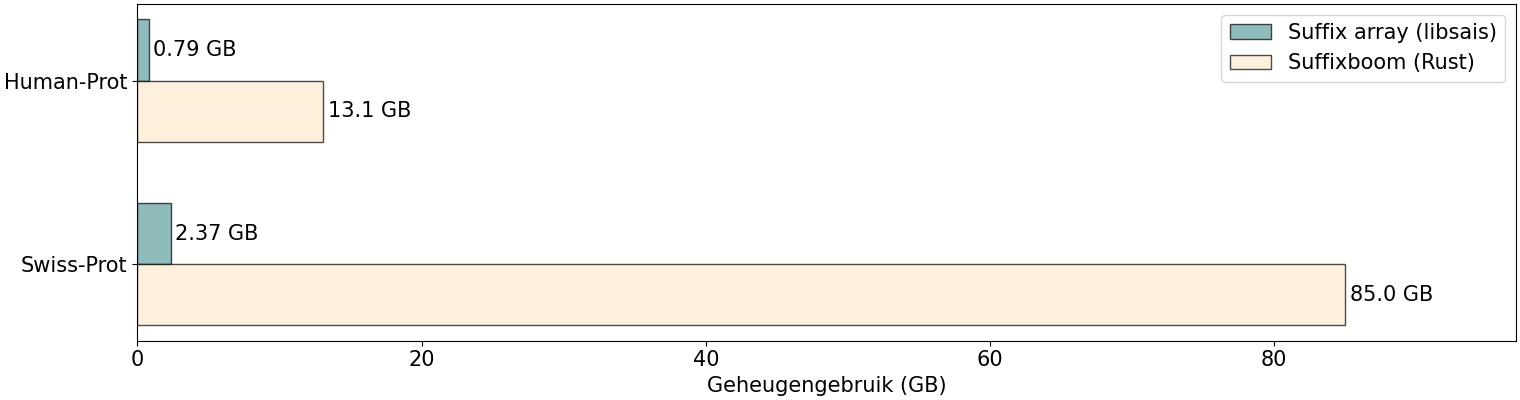
\includegraphics[width=\linewidth]{building_array_libsais_memory}}
    \caption{Vergelijking tussen de nodige tijd en hoeveelheid geheugen om een suffix array met LibSais of een suffixboom in onze eigen Rust implementatie op te bouwen. De tijd en het geheugengebruik zijn gemeten met het unix \texttt{time} commando. Als invoerbestand gebruiken we hier de Swiss-Prot of Human-Prot eiwitdatabank.}\label{fig:array_building}
\end{figure}

\subsection{Zoeken}
Aangezien er geen voorberekening gebeurt van LCA's is het enkel nuttig om de zoektijd inclusief het berekenen van de LCA te bekijken.
De tijd tot een match levert ons nog niet alle nodige informatie op, zoals dit het geval was bij de suffixboom.

\subsection{Beperken van het maximaal aantal matches}\label{subsec:maximaal-aantal-matches}
Op het eerste zicht lijkt de performantie voor sommige bestanden dramatisch veel slechter.
Dit is zichtbaar voor het Human-Prot peptidebestand in~\ref{fig:cutoff_humanprot}~(a).
Na wat onderzoek bleek dat het berekenen van de LCA* erg traag werd indien er een groot aantal matches was.
Daarom is er besloten om een \textbf{cut-off} in te stellen.
Indien een peptide meer dan dat aantal matches heeft, wordt verondersteld dat de root de kleinste gemeenschappelijke voorouder is van alle matches.
Uit onderzoek~\cite{unipept_cutoff} blijkt dat dit in de praktijk in de overgrote meerderheid van de gevallen ook effectief het geval is.
Zo zijn er slechts $\pm$ 13000 peptides die met meer dan 10000 eiwitten matchen.
Hierbij was voor 95\% van de peptides de LCA gelijk aan de root.
Slechts voor 200 peptides was er een resultaat op \textit{species} niveau.
\\
\begin{figure}[H]
    \centering
    \subfloat[Bereken de LCA* voor alle matches.]{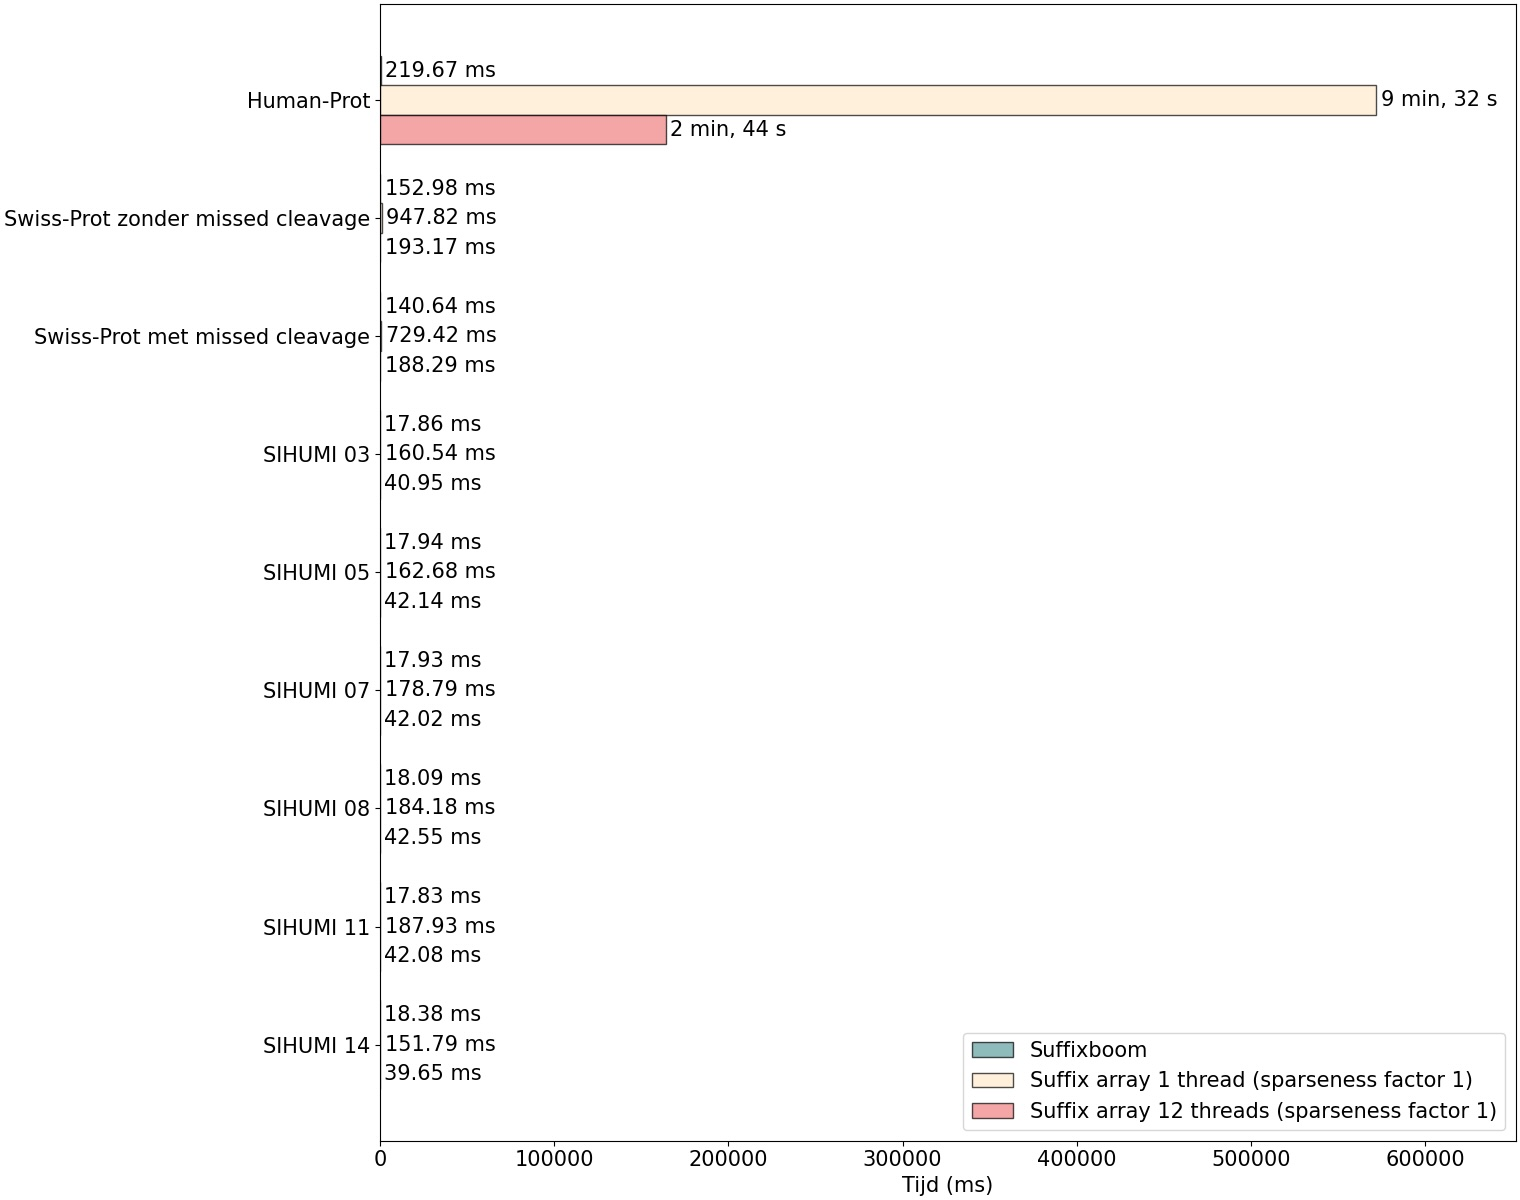
\includegraphics[width=0.7\linewidth]{no_cutoff_humanprot_search}}\\[4ex] % [4ex] om wat extra vertical spacing in te voegen

    \subfloat[Bereken de LCA* als er minder dan 10000 matches zijn.]{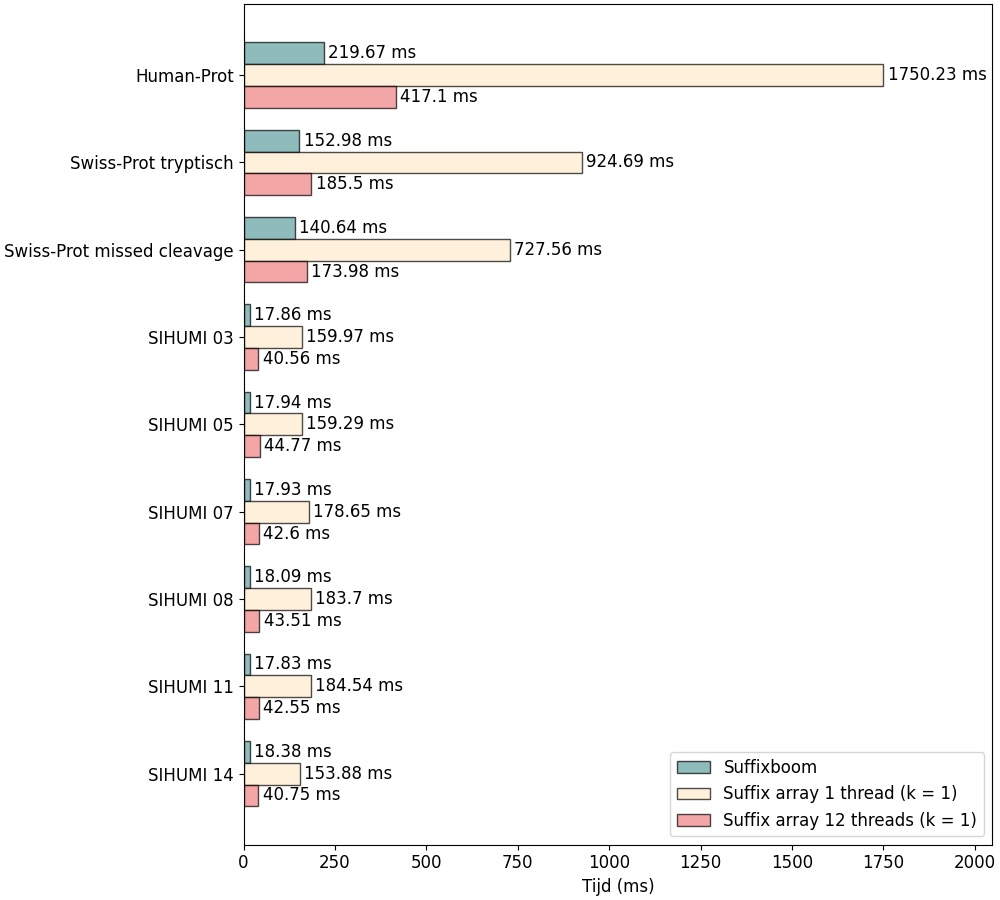
\includegraphics[width=0.7\linewidth]{cutoff_humanprot_search}}
    \caption{Berekenen van de LCA* (inclusief zoeken) voor alle peptiden in Human-Prot zonder en met cut-off.}\label{fig:cutoff_humanprot}
\end{figure}

In Figuur~\ref{fig:cutoff_humanprot} is duidelijk te zien dat de \textbf{uitvoeringstijd drastisch daalt} wanneer de cut-off op 10000 matches geplaatst wordt.
Als we dit specifiek bekijken voor de Human-Prot peptidebestanden en eiwitdatabank is de uitvoeringstijd maar liefst 300 keer sneller.
Bovendien is ook hier het \textbf{informatieverlies minimaal}.
Van de 250000 peptides zijn er 12 peptides die een ander resultaat verkrijgen in de output.
Deze 12 entries zijn echter slechts twee verschillende peptides (die gewoon meerdere malen voorkomen in het peptidebestand).
Dit zijn de peptides \texttt{EKP} en \texttt{SKE}.
Indien we de LCA* effectief berekenen is het resultaat in beide gevallen 9606, terwijl we met een cut-off de root (1) terug geven.
\\ \\
Nu we het zoeken in de suffix array afgesteld hebben aan de hand van een cut-off is het interessant om te kijken hoe de zoekperformantie zich verhoudt ten opzichte van het zoeken in een suffixboom.
In de praktijk is het zoeken in een suffix array 5 tot 10 maal trager voor onze testbestanden.
Een deel van deze extra zoektijd kan opgevangen worden door gebruik te maken van parallel zoeken.
Indien we hier gebruik van maken duurt het zoeken van 100\thinspace000 peptides op de Human-Prot en Swiss-Prot databank opnieuw enkele tientallen tot honderden milliseconden.
Natuurlijk zouden we het zoeken in een suffixboom ook kunnen parallelliseren.
Daarbij zal de absolute tijdswinst echter veel kleiner zijn doordat dit al zo snel is.

\section{Isoleucine en Leucine gelijkstellen}\label{sec:isoleucine-en-leucine-equivalentie}
Naast het vinden van exacte matches is het vinden van inexacte matches ook interessant.
Vooral het vinden van matches waarbij we een I (Isoleucine) en L (Leucine) aan elkaar gelijkstellen is een belangrijke optie in de huidige Unipept index.
\textbf{Deze twee aminozuren kunnen niet uit elkaar gehaald worden door een massaspectrometer vanwege hun identieke massa}.
Door deze restrictie van de huidige hardware is het voor onderzoekers erg nuttig om alle matches te vinden waar een I ook een L kan zijn of omgekeerd.
Om deze vorm van inexacte matching toe te voegen aan de index gebruik makende van een suffix array zijn meerdere opties.
\begin{enumerate}
    \item Bouw een extra index waarbij in de tekst elke L ook door een I vervangen wordt.
    Doe daarna hetzelfde in de peptides die we zoeken.
    Wanneer we in deze index de aangepaste peptides zoeken zullen we alle peptides vinden waar een I en L gelijkgesteld zijn.
    \item Genereer alle varianten van de gezochte peptide waarbij elke combinatie van I's en L'en gegenereerd wordt.
    Dit zal $2^i$ peptides genereren met $i$ het aantal I's en L'en in de peptide.
    \item Genereer de varianten van de gezochte peptide \textit{on the fly} tijdens het zoekproces.
    Hierbij kan gebruik gemaakt worden van het feit dat het binair zoeken naar een I en L hetzelfde patroon af legt tenzij bij een I, J, K of L\@.
    Dit zorgt ervoor dat voor een willekeurig patroon een groot stuk van de zoekboom gemeenschappelijk zal zijn.
    Bovendien zullen we tijdens het zoekproces een tak erg snel kunnen knippen.
    Dit is mogelijk wanneer op een bepaalde positie enkel een I of L beschikbaar is.
\end{enumerate}

De eerste aanpak is erg simpel en efficiënt.
Hierbij hebben we echter ook \textbf{dubbel zoveel geheugen} nodig om de index te hosten, en moeten we natuurlijk twee maal een suffix array opbouwen.
Het geheugenverbruik hiervoor verdubbelen is vrij drastisch, waardoor we we dit indien mogelijk willen vermijden.
\\ \\
De tweede aanpak is duidelijk ook erg simpel, en biedt veel \textbf{flexibiliteit}.
Zo is het bijvoorbeeld vrij simpel om algemenere karakterklasses te ondersteunen.
Het nadeel van deze aanpak is dat het \textbf{aantal te zoeken sequenties exponentieel stijgt met het aantal I's en L'en}, en daarmee dus ook de zoektijd.
Aangezien het ondersteunen van algemene karakterklasses ons te ver van ons doel leidt is dit iets waar we niet op focussen.
We willen specifiek snel I en L aan elkaar kunnen gelijkstellen, om zo de limitaties van de huidige massaspectrometers deels op te lossen.
\\ \\
Vanwege de mogelijke \textbf{optimalisaties tijdens het zoekproces} verkiezen wij de derde aanpak.
Hierbij is het echter belangrijk dat er ook bepaalde extreem slechte gevallen bestaan waarbij de zoekruimte erg groot wordt, en we niet efficiënt kunnen knippen.
De sequenties waarop we zoeken zijn namelijk niet random verdeeld over alle karakters van het alfabet.
Biologisch gezien komen bepaalde aminozuursequenties veel vaker voor.
Eén van deze patronen zijn de zogenaamde \textit{Leucine rich repeats}\cite{leucine_rich_repeats}.
Dit zijn sequenties waarin een reeks L'en in voorkomt.
In UniprotKB is bestaat er een \textbf{sequentie waar maar liefst 2397 L's na elkaar voorkomen}.
Dit is de proteïne met \textit{accession number} \texttt{A0A1Q9EZQ0}.
Wanneer we nu ook weten dat in UniProtKB ook reeksen aan I's voorkomen zorgt dit voor bepaalde extreem slechte gevallen.
Zo is hier \textbf{ook een proteïne met 641 opeenvolgende I's} (accession number: \texttt{A0A5J4P3H7}).
In het slechtste geval zou een gebruiker dus een sequentie van 641 I's of L'en kunnen insturen.
Dit zorgt ervoor dat we in de zoekboom $2^{641} \approx 9.12^{192}$ opties moeten proberen.
Het grootste aandeel van deze opties zal niet voorkomen, waardoor de takken van deze boom allemaal extreem kort zullen zijn.
Dit zal echter verwaarloosbaar zijn ten opzichte van het gigantisch aantal opties.
Om dit in perspectief te plaatsen: Men schat dat er in het totaal $10^{79}$ atomen in het universum zijn~\cite{atoms_in_universe} en dat het universum ongeveer $4.36^{20}$ milliseconden oud is~\cite{age_universe}.
Zelfs als het controleren van één optie minder dan een milliseconde duurt zou dit dus nog onmogelijk zijn.
\textbf{Om de zoektijd en het geheugenverbruik te beperken, hebben we ervoor gekozen om twee vormen van restricties op te leggen wanneer I en L gelijkgesteld worden}.
\begin{enumerate}
    \item Laat maximaal 5 seconden aan zoektijd per peptide toe.
    \item Laat per peptide in het totaal maximaal 34 I's en L'en toe.
\end{enumerate}
Deze twee restricties samen moeten de servers deels helpen beschermen tegen Denial of Service attacks.
In de praktijk wordt normaal de tijdslimiet van 5 seconden eerst bereikt.
Dit vertaalt zich naar een sequentie van ongeveer 25 I's of L'en.
Elke keer we één extra teken zouden willen toelaten verdubbelt de zoektijd.
Zo duurt het al één minuut om een sequentie met 30 opeenvolgende I's of L'en te zoeken.
Wanneer we echter nog veel meer I's of L'en toelaten stuiten we vrij snel op een geheugenlimiet.
Om te voorkomen dat het programma meer geheugen probeert te vragen dan dat de server heeft, waarna het crasht.
Hebben we beslist maximaal 34 I's of L'en toe te laten.
In het slechte geval gebruikt één enkele thread hierbij iets meer dan 2 GB RAM\@.
Aangezien het zoeken multithreaded is, moeten we dus een goede 20 GB aan vrij geheugen voorzien wanneer de index ingeladen is.
\textbf{Wanneer we deze limieten testen door alle test peptidebestanden te zoeken in de volledige UniProtKB databank worden deze limieten geen enkele keer geraakt}.
\\ \\
\textbf{In de praktijk} vertaalt het gelijkstellen van I en L aan de hand van de derde optie zich naar een \textbf{vrij kleine overhead}.
Deze beperkte overhead valt te zien in Figuur~\ref{fig:uniprot_search}.

\section{UniProtKB}\label{sec:uniprotkb}
Zoals eerder vermeld levert een ruwe extrapolatie op dat we $\pm$ 1.2 TB aan geheugen nodig zou hebben om een index voor UniProtKB op te bouwen.
Hierbij werd er echter van uitgegaan dat UniProtKB 500x meer eiwitten dan Swiss-Prot bevat.
Dit is een overschatting van de realiteit waar UniProt op dit moment \textit{slechts} $\pm$ 440 keer groter is.
Dit zorgt ervoor dat het opbouwen mogelijks al \textbf{haalbaar is op HPC van UGent} waar nodes beschikbaar zijn die ongeveer 940 GB aan beschikbaar geheugen hebben.
Na dit te proberen bleek \textit{slechts} 740 GB RAM nodig.
Figuur~\ref{fig:build_uniprot} toont de nodige tijd en hoeveelheid geheugen om dit te realiseren.
\textbf{Opvallend hierbij is dat het libsais algoritme hier trager is dan libdivsufsort}, terwijl dit voor alle kleinere datasets net omgekeerd was.
Afhankelijk van je dataset is het ene algoritme dus sneller dan het andere.
Het geheugengebruik van beide algoritmes blijft echter erg gelijkaardig, wat het belangrijkste is voor ons.
\\
\begin{figure}[H]
    \centering
    \subfloat[Tijd nodig om een index voor UniProtKB te bouwen.]{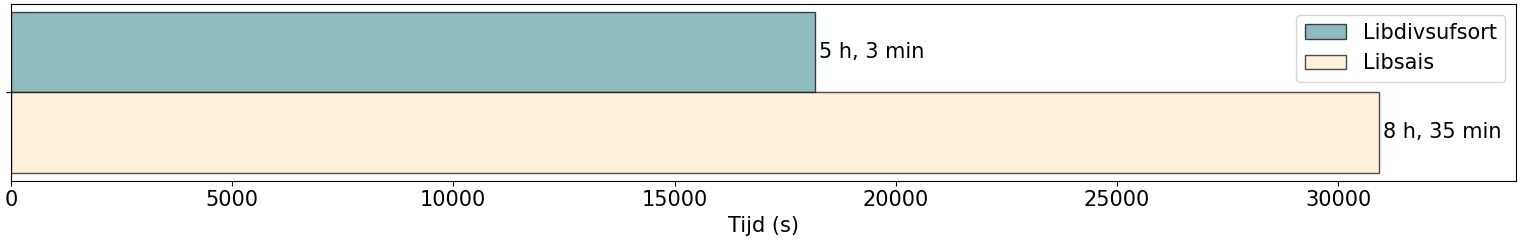
\includegraphics[width=\linewidth]{build_uniprot_time}}\\[4ex] % [4ex] om wat extra vertical spacing in te voegen

    \subfloat[Maximale hoeveelheid geheugen gebruikt tijdens het opbuowen van een index voor UniProtKB.]{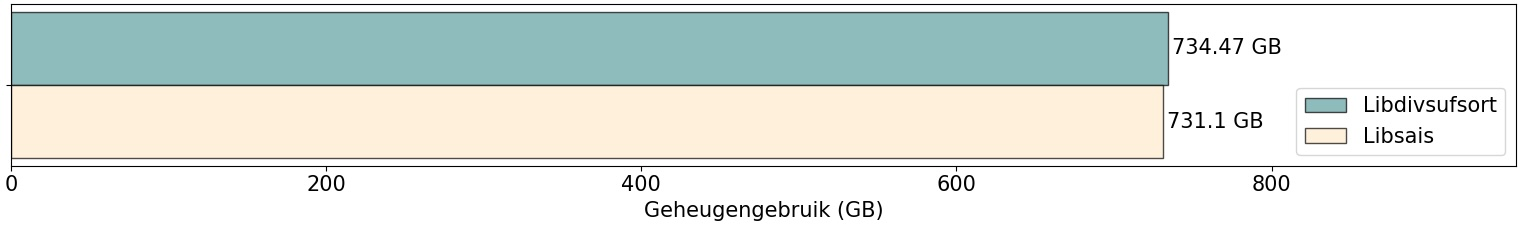
\includegraphics[width=\linewidth]{build_uniprot_memory}}
    \caption{Statistieken voor het opbouwen van een SA voor UniProtKB}\label{fig:build_uniprot}
\end{figure}

Een volgende stap na het opbouwen van de volledige SA was het beslissen van de sparseness factor.
Zoals eerder aangegeven in de conclusie van sectie~\ref{subsec:zoeken-in-sparse-suffix-arrays} willen we deze sparseness factor zo laag mogelijk kiezen, met als restrictie dat de SSA nog steeds in het geheugen moet kunnen gehouden worden.
De beschikbare machines die UniPept hosten hebben elk $pm$ 0.5 TB RAM ter beschikking.
Dit wil zeggen dat we de resulterende index hierin moeten krijgen, en ook nog genoeg overhead moeten laten zodat de machine zeker niet out-of-memory gaat tijdens het hosten van de index en het verwerken van meerdere requests.
Praktisch gezien komt dit er op neer dat we gebruik maken van \textbf{sparseness factor 3}.
Dit resulteert in een SA van 231.81 GB\@.
In combinatie met de tekst (86.93 GB) resulteert dit in een \textbf{totale indexgrootte van 318.74 GB}, wat comfortabel in de 0.5 TB past.
Hierbij moet natuurlijk nog wat overhead gerekend worden om de mapping van de suffix naar proteïne bij te houden.
Bovendien bevatten deze servers ook nog andere databanken om verdere aggregaties te berekenen.
Zo biedt Unipept naast een taxonomische analyse ook nog een functionele analyse aan.
Deze functionele analyse wordt uitgevoerd op basis van de gematchte eiwitten die de indexstructuur terug geeft.
Indien we sparseness factor 2 zouden gebruiken komt de totale indexgrootte uit op $\pm$ 450 GB\@.
Dit op zich zou nog net in de machine passen, maar laat niet genoeg ruimte voor de andere processen.
\\ \\
Natuurlijk is naast het effectief kunnen in het geheugen houden van de indexstructuur de zoekperformantie extreem belangrijk.
Zoals verwacht op basis van de kleinere testen is deze nog steeds goed.
Figuur~\ref{fig:uniprot_search} toont de resultaten voor onze testbestanden.

\begin{figure}[ht]
    \centering
    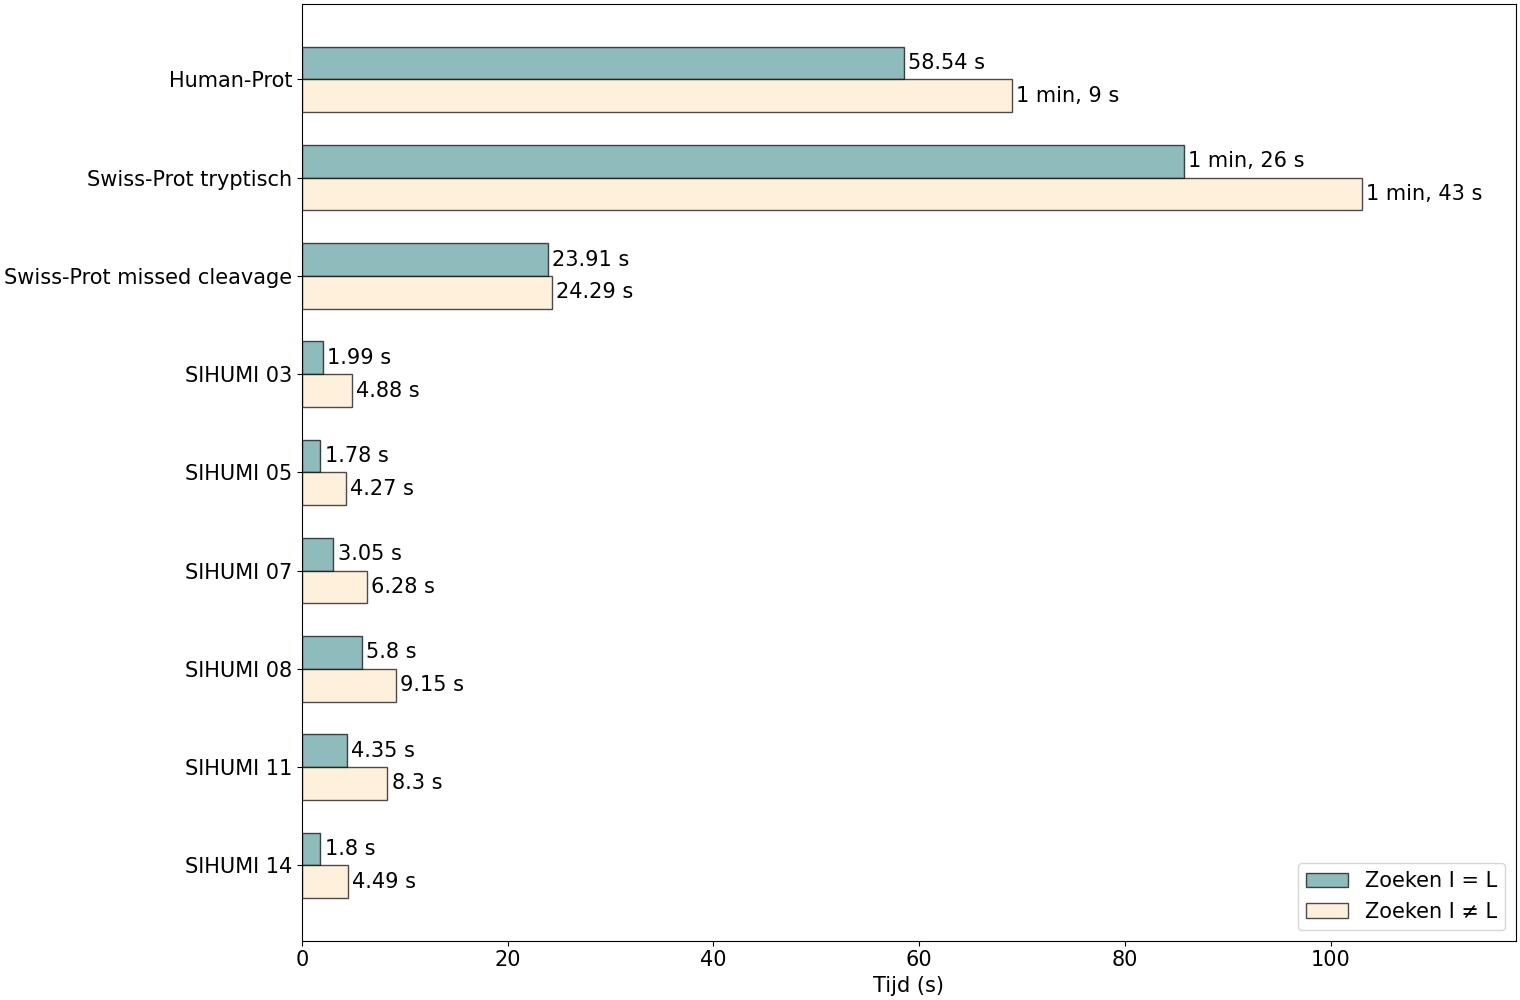
\includegraphics[width=0.95\linewidth]{uniprot_searchtime_standard_vs_il_equality}
    \caption{Zoektijd op Uniprot (Swiss-Prot + TrEMBL) met en zonder het gelijkstellen van I en L op een SA met sparseness factor 3.}
    \label{fig:uniprot_search}
\end{figure}

\subsection{Vergelijking met andere tools}\label{subsec:vergelijking-met-andere-tools}
Aangezien we er in geslaagd zijn om UniProtKB volledig te indexeren is het nuttig om de performantie te vergelijken met bestaande tools.
De tools die we bekijken zijn de \textbf{Uniprot Peptide search tool}, de \textbf{Expasy ScanProsite tool} en \textbf{Unipept} (met de bestaande indexstructuur).
Vanwege de performantie zullen we ons beperken tot het opzoeken van één willekeurige peptide \texttt{ISPAVLFVIVILAVLFFISGLLHLLVR}.
Als referentie gebruiken we de zoektijd in de nieuwe indexstructuur gebruikmakende van een suffix array met sparseness factor 3.
Hierin duurt het zoeken van de peptide \textbf{0.01 seconden} en levert 50 matches op.
Wanneer we I en L gelijkstellen duurt dit opnieuw 0.01 seconden, maar levert dit wel 52 matches op.
Hierbij wordt natuurlijk geen extra tijd geïntroduceerd door een API call over het internet aangezien deze index (nog) niet publiek beschikbaar is.

\subsubsection{UniProt peptide search tool}
De UniProt peptide search tool\cite{uniprot_search_paper, uniprot_search_site} is een onderdeel van de UniProt site en laat toe om alle voorkomens van een bepaald eiwit te vinden in de volledige UniProtKB database.
Als opties kunnen we kiezen om enkel in Swiss-Prot te zoeken, of in Swiss-Prot en TrEMBL.
Voor beide datasets kunnen we kiezen of we I en L aan elkaar willen gelijkstellen.
Deze features komen exact overeen met de eigenschappen van onze nieuwe indexstructuur.
Qua performantie heeft deze tool echter meerdere problemen.
Zo duurt het zoeken (zonder het gelijkstellen van I en L) op Swiss-Prot + TrEMBL ongeveer \textbf{20 minuten}.
Wanneer we I en L aan elkaar gelijkstellen duurt het zoeken ongeveer 10 minuten, en vinden we dezelfde 52 matches zoals uit de nieuwe index.
Deze uitvoeringstijden zijn echter extreem variabel.
Zo is hier vermoedelijk een vorm van caching toegepast aangezien het zoeken voor een tweede keer extreem veel sneller gaat.
Dit maakt het benchmarken extreem moeilijk.
Naast de variabele performantie faalt deze tool ook regelmatig tijdens het berekenen en ophalen van de resultaten.


\subsubsection{Expasy ScanProsite tool}
De Expasy ScanProsite tool\cite{scanprosite} laat toe om aan de hand van een taaltje die lijkt op reguliere expressies allerlei patronen te zoeken.
Hun eigen taal laat toe om onder andere wildcards, karakterklasses, inverse klasses en herhalingen te specificeren.
De flexibiliteit van dit systeem is dus een sterk voordeel.
Een nadeel van deze tool is dat niet de volledige UniProtKB databank doorzocht wordt.
Er wordt enkel rekening gehouden met proteïnes die deel uit maken van een reference proteome\footnote{Deze zogenaamde reference proteomes zijn een collectie van eiwitten die door een bepaald organisme gemaakt kunnen worden, en die bovendien taxonomisch belangrijk bevonden worden. Deze laatste voorwaarde wil dus zeggen dat dit niet zomaar van elk organisme is, enkel van een selecte groep organismes die op basis van verschillende factoren belangrijk bevonden wordt. Een voorbeeld hiervan is de \textit{human reference proteome}. Dit zijn alle eiwitten die door een mens aangemaakt kunnen worden.}.
Dit komt er op neer dat ze bij UniProt 2024\_01 \textbf{slechts rekening houden met 85\thinspace152\thinspace388 van de 249\thinspace751\thinspace891 proteïnes}.
Wanneer we de zoekperformantie hier testen duurt het zoeken van de ene peptide zo'n \textbf{5.5 minuten} zonder gelijkstellen van I en L en 15 minuten met het gelijkstellen van I en L\@.
Hierbij zijn er slechts 30 resp. 32 matches gevonden, wegens de subset van proteïnes die gebruikt wordt.

\subsubsection{Huidige Unipept index}
De bestaande Unipept index laat toe om, \textbf{op voorwaarde dat je peptide tryptisch is}, alle matches te vinden met de keuze om I en L gelijk te stellen.
De peptide die we hier gebruiken is dit ook net, dus zou deze index hiervoor dezelfde matches moeten vinden.
Dit is inderdaad het geval, en gebeurt bovendien gebruik makende van een API call in \textbf{0.1 seconden}, wat duidelijk extreem veel sneller is dan de andere bestaande opties.
Opnieuw is de zoektijd hier al zo klein dat de invloed van het gelijkstellen van I en L niet te meten valt.
Dat dit enkel werkt voor tryptische peptides is een extreem grote beperking, volgend voorbeeld illustreert dit.
Stel dat we nu de peptide \texttt{ILAKLFIS} zoeken.
Dit is geen tryptische peptide en bijgevolg kunnen er geen matches gevonden worden.
De nieuwe indexstructuur vindt echter 14 matches zonder I en L gelijk te stellen, en 207 matches bij het gelijkstellen van I en L.

\section{Aanbieden van de nieuwe indexstructuur}\label{sec:aanbieden-van-de-nieuwe-indexstructuur}
Alle eerder vermelde benchmarks tonen enkel de zoektijd.
Bij het opstarten moeten we echter \textbf{eerst de indexstructuur inladen}.
Dit alleen duurt 20 tot 25 minuten.
We willen dit inladen slechts eenmalig doen om dan alle requests onmiddellijk af te kunnen afhandelen.
Dit doen we aan de hand van een simpele webserver aan de hand van de Axum crate\cite{axum}.
Deze webserver laadt bij het opstarten de indexstructuur in en blijft daarna wachten op HTTP requests die een JSON bevatten met daarin de peptides die we willen zoeken.
Op deze manier is dit probleem elegant opgelost, en kunnen we bovendien aan de hand van JSON bestanden erg makkelijk de input verwerken, en de resultaten terugsturen.


